\section{Παρουσίαση προσωπικών δεδομένων εργασίας}

Τα δεδομένα που αφορούν γεωμετρικές παραμέτρους και φυσικά μεγέθη παρατίθενται στον πίνακα \ref{tab:data}.

\begin{table}[h!]
    \begin{center}
        \begin{tabular}[c]{|c|c|}
            \hline
            k & 0.09 \\
            a & 0.216 \\
            b & 1.03 \\
            c & 0.97 \\
            $p_{\text{αεροφ}}$ & 4 bar\\
            $p_{\text{εξ}}$ & 3.3 bar\\
            $T_{\text{αεροφ}}$ & 286Κ\\
            Μήκος αγωγού & 2m\\
            \hline
        \end{tabular}
    \end{center}
    \caption{Δεδομένα εργασίας}
    \label{tab:data}
\end{table}

Η τιμή της πυκνότητας για τις συνοριακές συνθήκες και για την αρχικοποίηση υπολογίζονται ως $\rho = \dfrac{p}{RT}$.

Αντίστοιχα, οι αριθμητικές παράμετροι που χρησιμοποήθηκαν παρατίθενται στον πίνακα \ref{tab:num}.

\begin{table}[h!]
    \begin{center}
        \begin{tabular}[c]{|c|c|}
            \hline
            Αριθμός κόμβων & 801 \\
            Χρονικό βήμα & $10^{-6}s$ \\
            Αριθμός βημάτων & 45000 \\
            Τελικός χρόνος & 0.045s \\
            \hline
        \end{tabular}
    \end{center}
    \caption{Αριθμητικές παράμετροι}
    \label{tab:num}
\end{table}

Η τάξη μεγέθους του χρονικού βήματος επιλέχθηκε ακολουθώντας το όριο του Courant. Ο αριθμός του Courant είναι:

\begin{equation*}
   C = \dfrac{Udt}{dx} 
\end{equation*}

Ο αριθμός Courant θέλουμε να είναι τουλάχιστον μικρότερος της μονάδας, αλλά συνήθως θέλουμε να είναι αρκετά μικρότερος. Λύνωντας ως προς dt έχουμε:

$$ dt = \dfrac{Cdx}{U}$$

Αν θεωρήσουμε πως η ταχύτητα μπορεί να φτάσει περίπου 2 φορές την ταχύτητα του ήχου ($\approx 600m\s$) και αριθμό Courant C = 0.5, τότε προκύπτει οτι θέλουμε το χρονικό βήμα να είναι περίπου τρεις τάξεις μεγέθους μικρότερο απο το χωρικό βήμα. Έτσι ακολουθήσαμε αυτό τον κανόνα για την επιλογή του χρονικού βήματος.

Ο αριθμός των κόμβων (αντίστοιχα μήκος κελλιού) επιλέχθηκε με δοκιμές, ξεκινώντας απο μικρό αριθμό αυξάνοντας σταδιακά έως να ευσταθήσει η σύγκλιση του κώδικα.


\subsection{Γεωμετρία αγωγού}[h!]

Με βάση τα αριθμητικά δεδομένα που παρουσιάστηκαν στον πίνακα \ref{tab:data}, η γεωμετρία που προκύπτει φαίνεται στο σχήμα \ref{fig:geometry}.

\begin{figure}[h!]
    \begin{center}
        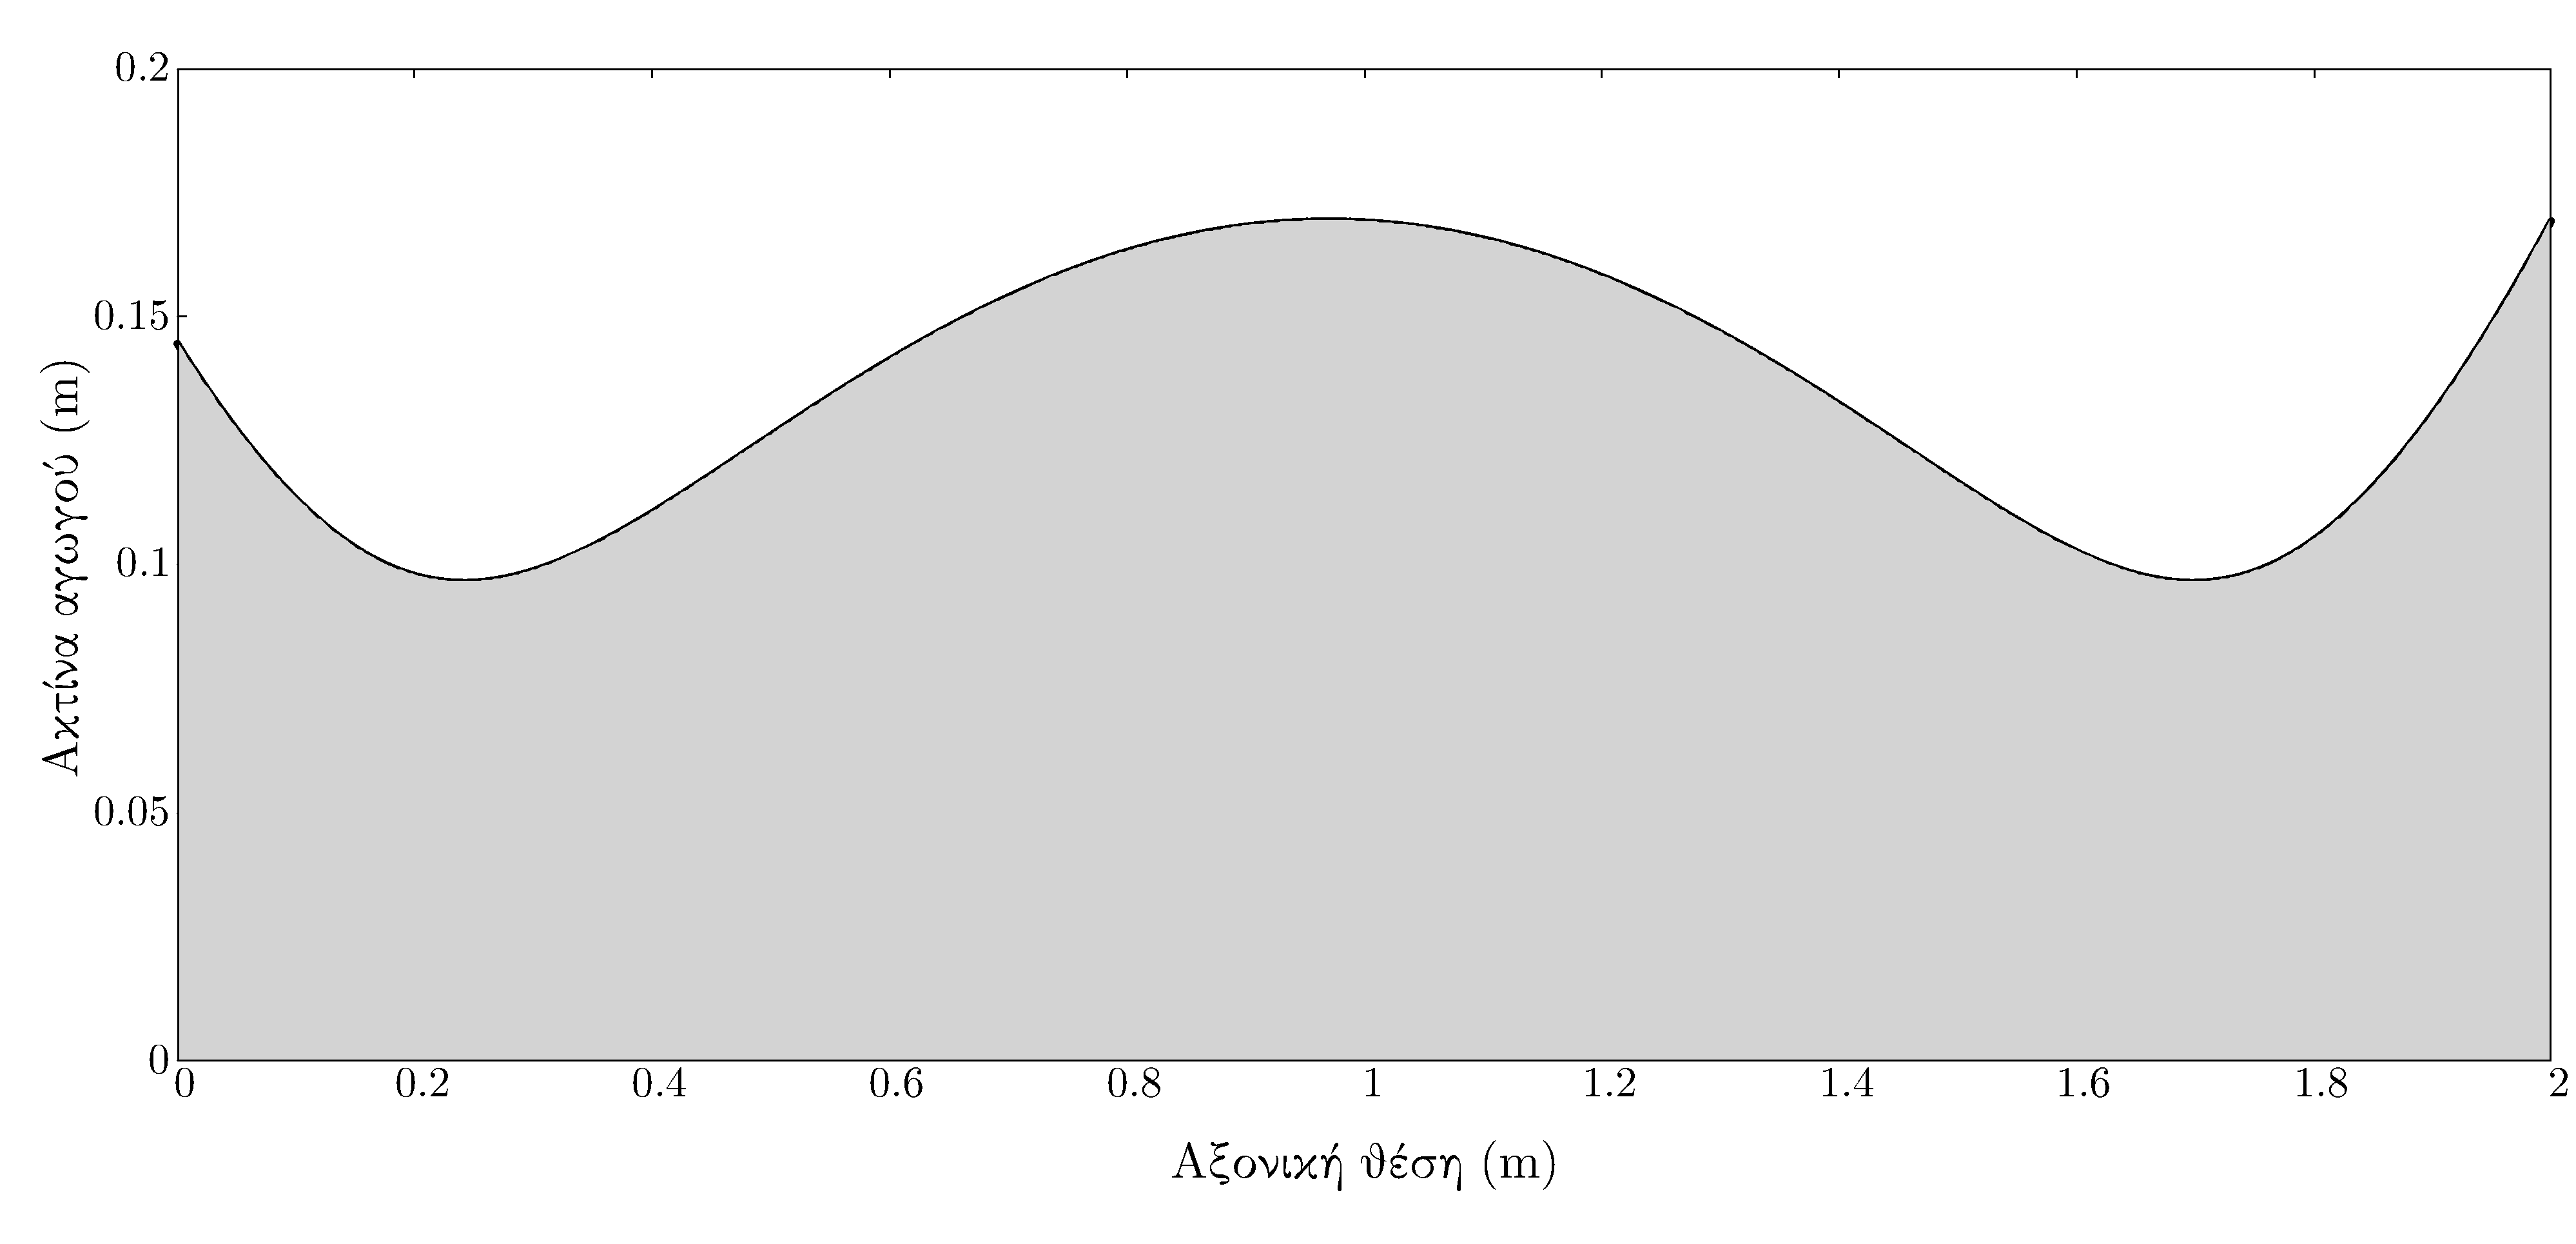
\includegraphics[width=0.85\textwidth]{figures/tube_diam.pdf}
    \end{center}
    \caption{Διάγραμμα μεταβολής ακτίνας αγωγού}
    \label{fig:geometry}
\end{figure}


